\subsection{Ausfüllrätsel}
Im vorangegangenen Abschnitt haben wir \textsl{SUDOKU} auf \textsl{SAT}
reduziert.
Ein \textsl{SUDOKU}-Problem wurde in eine Formel verwandelt, die genau
dann erfüllbar war, wenn das \textsl{SUDOKU}-Rätsel lösbar war.
In diesem Abschnitt zeigen wir, dass diese Idee viel allgemeiner ist.

\begin{figure}
\centering
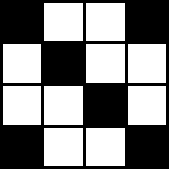
\includegraphics{images/ausfuell-1.pdf}
\qquad
\qquad
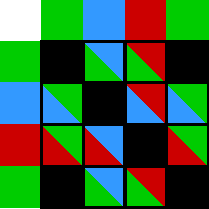
\includegraphics{images/ausfuell-2.pdf}
\caption{Ausfüllrätsel zum Grapheinfärbeproblem aus
Abbildung~\ref{vertex-coloring-examples}, links das leere `Spielfeld',
rechts ausgefüllt mit den Farben der Knoten.
\label{ausfuell:coloring}}
\end{figure}
Sehr viele Rätsel werden auf einem rechteckigen Feld von Zellen
bespielt, in die man etwas eintragen muss.
Sogar das Graphenfärbeproblem (\textsl{VERTEX-COLORING}) kann man
so auffassen.
Dazu formt man den gegebenen Graphen mit $n$ in eine
$n\times n$-Tabelle um, die Zeilen und Spalten entsprechen den Knoten
des Graphen, die Felder den möglichen Kanten.
Alle Felder, die zu im Graphen nicht existierenden Kanten gehören,
werden schwarz gefärbt.
In die weissen Felder müssen jetzt Paare von verschiedenen Farben
eingetragen werden, so dass in jeder Zeile die erste Farbe immer
gleich ist, und in jeder Spalte die zweite Farbe.
Ausserdem muss die Farbe einer Spalte und der entsprechenden Zeile
gleich sein.
Der Graph ist einffärbbar, wenn es möglich ist, die Tabelle wie
beschrieben auszufüllen (Abbildung~\ref{ausfuell:coloring}).

\begin{definition}
Ein {\em polynomielles Ausfüllrätsel} ist eine $n\times m$-Tabelle,
in die Zeichen eines Alphabets $\Sigma$ eingefüllt werden müssen,
so dass gewisse Regeln eingehalten werden. 
Die einzuhaltenden Regeln können durch eine logische Formel beschrieben
werden, die in einer Zeit polynomiell in $nm$ berechnet werden kann.
\end{definition}

Die Bedingung der Berechenbarkeit in polynomieller Zeit ist meistens
offensichtlich.
Oft entsteht die Formel nämlich durch Anpassung der immer gleichen
Regeln für jedes Feld.
In solchen Fällen genügt es, wenn die resultierende Formel polynomielle
Länge hat.

\begin{beispiel}
Die Formel, die die Sudoku-Regeln für das $n^2\times n^2$-beschreibt,
besteht aus einer 
Teilformel für jedes Feld, welche wiederum aus einer Teilformel
für Zeilen, Spalten und Unterfelder besteht.
Diese Teilformeln überprüfen die Werte aller $n^2$ Felder der Zeile,
Spalte oder des Unterfeldes, dabei sind $n^2$ mögliche Feldinhalte
zu berücksichtigen.
Im Abschnitt~\ref{subsection:sudoku-und-sat} wurde gezeigt, wie die
Teilformel aufzubauen ist, ihre Länge ist
\[
O(\underbrace{n^2}_{\text{Vergleichsfelder}}\cdot
\underbrace{n^2}_{\text{Zeichen}}) = O(n^4).
\]
Die gesamte Formel hat damit die Länge
\[
O(\underbrace{n^4}_{\text{Felder}}\cdot
\underbrace{n^2}_{\text{Vergleichsfelder}}\cdot
\underbrace{n^2}_{\text{Zeichen}}) = O(n^8).
\]
Insbesondere ist die Länge der Formel polynomiell in der Feldgrösse $n^4$,
\textsl{SUDOKU}
ist also ein polynomielles Ausfüllrätsel im genannten Sinn.
\end{beispiel}

\begin{satz}
Ein polynomielles Ausfüllrätsel $A$ lässt sich polynomiell auf 
\textsl{SAT} reduzieren.
\end{satz}

\begin{proof}[Beweis]
Polynomielle Reduktion auf \textsl{SAT} bedeutet, dass man zu jeder
Probleminstanz eine logische Formel $\varphi$ konstruieren muss,
deren Länge polynomiell in der Grösse des Ausgangsproblems ist.
Die Formel muss genau dann erfüllbar sein, wenn das ursprüngliche
Problem lösbar ist.
Ein polynomielles Ausfüllrätsel führt aber nach Definition auf
eine solche Formel.
\end{proof}

Als Konsequenz dieser Konstruktion können wir auch schliessen, dass
jedes Ausfüllrätsel in NP liegt.

